% Generated from reviewed lane; compile via book/textbook.tex.
\clearpage

原书 PDF 页 215；印刷页码 202。

\href{source-images/pdf-215.jpeg}{原页图像}

\section{第 8 章　解线性方程组的迭代法}\label{ch08-ux7b2c-8-ux7ae0-ux89e3ux7ebfux6027ux65b9ux7a0bux7ec4ux7684ux8fedux4ee3ux6cd5}

\subsection{8.1　引言}\label{ch08-ux5f15ux8a00}

考虑线性方程组

\[
Ax=b,
\tag{8.1.1}
\]

其中 \(A\) 为非奇异矩阵。当 \(A\) 为低阶稠密矩阵时，第 7 章所讨论的选主元素消去法是解式（8.1.1）的有效方法。但是，对于由工程技术中产生的大型稀疏矩阵方程组（\(A\) 阶数 \(n\) 很大，但零元素较多，例如 \(n\geqslant10^4\)，由某些偏微分方程数值解所产生的线性方程组），利用迭代法求解式（8.1.1）是合适的。在计算机内存和运算两方面，迭代法通常都可利用 \(A\) 中有大量零元素的特点。

本章将介绍迭代法的一些基本理论及 Jacobi 迭代法、Gauss-Seidel 迭代法、超松弛迭代法。超松弛迭代法应用很广泛。

下面举简例，以便了解迭代法的思想。

\textbf{例 8.1}　求解方程组

\[
\begin{cases}
8x_1-3x_2+2x_3=20,\\
4x_1+11x_2-x_3=33,\\
6x_1+3x_2+12x_3=36,
\end{cases}
\tag{8.1.2}
\]

记作

\[
Ax=b,
\]

其中

\[
A=\begin{bmatrix}8&-3&2\\4&11&-1\\6&3&12\end{bmatrix},\qquad
x=\begin{bmatrix}x_1\\x_2\\x_3\end{bmatrix},\qquad
b=\begin{bmatrix}20\\33\\36\end{bmatrix}.
\]

方程组的精确解是

\[
x^*=(3,2,1)^{\mathrm T}.
\]

现将式（8.1.2）改写成

\[
\begin{cases}
x_1=\dfrac18(3x_2-2x_3+20),\\[4pt]
x_2=\dfrac1{11}(-4x_1+x_3+33),\\[4pt]
x_3=\dfrac1{12}(-6x_1-3x_2+36)
\end{cases}
\tag{8.1.3}
\]

\clearpage

原书 PDF 页 216；印刷页码 203。

\href{source-images/pdf-216.jpeg}{原页图像}

或

\[
x=B_0x+f,
\]

其中

\[
B_0=\begin{bmatrix}
0&\dfrac38&-\dfrac28\\[4pt]
-\dfrac4{11}&0&\dfrac1{11}\\[4pt]
-\dfrac6{12}&-\dfrac3{12}&0
\end{bmatrix}=I-D^{-1}A,\qquad
f=\begin{bmatrix}\dfrac{20}8\\[4pt]\dfrac{33}{11}\\[4pt]\dfrac{36}{12}\end{bmatrix}=D^{-1}b.
\]

任取初始值，例如取 \(x^{(0)}=(0,0,0)^{\mathrm T}\)。将这些值代入式（8.1.3）右端（若式（8.1.3）为等式即求得方程组的解，但一般不满足），得到新的值

\[
x^{(1)}=(x_1^{(1)},x_2^{(1)},x_3^{(1)})^{\mathrm T}=(2.5,3,3)^{\mathrm T},
\]

再将 \(x^{(1)}\) 分量代入式（8.1.3）右端，得到 \(x^{(2)}\)。反复利用这个计算程序，得到一向量序列和一般的计算公式（迭代公式）

\[
x^{(0)}=\begin{bmatrix}x_1^{(0)}\\x_2^{(0)}\\x_3^{(0)}\end{bmatrix},\quad
x^{(1)}=\begin{bmatrix}x_1^{(1)}\\x_2^{(1)}\\x_3^{(1)}\end{bmatrix},\quad\cdots,\quad
x^{(k)}=\begin{bmatrix}x_1^{(k)}\\x_2^{(k)}\\x_3^{(k)}\end{bmatrix},\quad\cdots,
\]

\[
\begin{cases}
x_1^{(k+1)}=(3x_2^{(k)}-2x_3^{(k)}+20)/8,\\
x_2^{(k+1)}=(-4x_1^{(k)}+x_3^{(k)}+33)/11,\\
x_3^{(k+1)}=(-6x_1^{(k)}-3x_2^{(k)}+36)/12,
\end{cases}
\tag{8.1.4}
\]

简写为

\[
x^{(k+1)}=B_0x^{(k)}+f,
\]

其中 \(k\)（\(k=0,1,2,\cdots\)）表示迭代次数。

迭代到第 10 次有

\[
x^{(10)}=(3.000\,032,\ 1.999\,838,\ 0.999\,881\,3)^{\mathrm T},
\]

\[
\|\varepsilon^{(10)}\|_\infty=0.000\,187\quad(\varepsilon^{(10)}=x^{(10)}-x^*).
\]

从此例看出，由迭代法作出的向量序列 \(x^{(k)}\) 逐步逼近方程组的精确解 \(x^*\)。

对于任何一个方程组 \(x=Bx+f\)（由 \(Ax=b\) 变形得到的等价方程组），按迭代法作出的向量序列 \(x^{(k)}\) 是否一定逐步逼近方程组的解 \(x^*\) 呢？回答是不一定。请读者考虑，用迭代法解下述方程组

\[
\begin{cases}
x_1=2x_2+5,\\
x_2=3x_1+5.
\end{cases}
\]

对于给定方程组 \(x=Bx+f\)，设有唯一解 \(x^*\)，则

\[
x^*=Bx^*+f.
\tag{8.1.5}
\]

又设 \(x^{(0)}\) 为任取的初始向量，按下述公式构造向量序列

\[
\begin{cases}
x^{(1)}=Bx^{(0)}+f,\\
x^{(2)}=Bx^{(1)}+f,\\
\qquad\vdots\\
x^{(k+1)}=Bx^{(k)}+f,
\end{cases}
\tag{8.1.6}
\]

\begin{quote}
校注（agent 补充）：原页将 \(x^{(10)}\) 的第二分量印为 \(1.999\,838\)，误差范数印为 \(0.000\,187\)，均按原样保留。由式（8.1.4）从 \(x^{(0)}=0\) 作 10 次有理数迭代，所得向量约为 \((3.0000318141,1.9998740186,0.9998812605)^{\mathrm T}\)，实际误差的无穷范数约为 \(0.0001259814\)；即使按本页印刷的三个分量计算，误差无穷范数也应为 \(0.000162\)。第二分量及误差范数疑为原书数值错误，并非 OCR 错误。
\end{quote}

\clearpage

原书 PDF 页 217；印刷页码 204。

\href{source-images/pdf-217.jpeg}{原页图像}

其中 \(k\) 表示迭代次数。

\textbf{定义 8.1}　\(1^\circ\) 对于给定的方程组 \(x=Bx+f\)，用式（8.1.6）逐步代入求近似解的方法称为\textbf{迭代法}（或称为一阶定常迭代法，这里 \(B\) 与 \(k\) 无关）。

\(2^\circ\) 如果 \(\lim\limits_{k\to\infty}x^{(k)}\) 存在（记作 \(x^*\)），称此迭代法\textbf{收敛}，显然 \(x^*\) 就是方程组的解，否则称此迭代法\textbf{发散}。

由上述讨论，需要研究 \(\{x^{(k)}\}\) 的收敛性。引进误差向量

\[
\varepsilon^{(k+1)}=x^{(k+1)}-x^*,
\]

由式（8.1.6）减去式（8.1.5），得

\[
\varepsilon^{(k+1)}=B\varepsilon^{(k)}\quad(k=0,1,2,\cdots),
\]

递推得

\[
\varepsilon^{(k)}=B\varepsilon^{(k-1)}=\cdots=B^k\varepsilon^{(0)}.
\]

要考察 \(\{x^{(k)}\}\) 的收敛性，就要研究 \(B\) 在什么条件下有 \(\varepsilon^{(k)}\to0\)（\(k\to\infty\)），亦即要研究 \(B\) 满足什么条件时有 \(B^k\to O\)（零矩阵）（\(k\to\infty\)）。

\subsection{8.2　Jacobi 迭代法与 Gauss-Seidel 迭代法}\label{ch08-jacobi-ux8fedux4ee3ux6cd5ux4e0e-gauss-seidel-ux8fedux4ee3ux6cd5}

\subsubsection{8.2.1　Jacobi 迭代法}\label{ch08-jacobi-ux8fedux4ee3ux6cd5}

设有方程组

\[
\sum_{j=1}^n a_{ij}x_j=b_i\quad(i=1,2,\cdots,n),
\]

记作

\[
Ax=b,
\tag{8.2.1}
\]

\(A\) 为非奇异阵且 \(a_{ij}\neq0\)（\(i=1,2,\cdots,n\)）。将 \(A\) 分裂为 \(A=D-L-U\)，其中

\[
D=\begin{bmatrix}
a_{11}&&&&\\
&a_{22}&&&\\
&&\ddots&&\\
&&&\ddots&\\
&&&&a_{nn}
\end{bmatrix},\qquad
L=-\begin{bmatrix}
0&&&&\\
a_{21}&0&&&\\
a_{31}&a_{32}&0&&\\
\vdots&\vdots&\ddots&\ddots&\\
a_{n1}&a_{n2}&\cdots&a_{n,n-1}&0
\end{bmatrix},
\]

\[
U=-\begin{bmatrix}
0&a_{12}&a_{13}&\cdots&a_{1n}\\
&0&a_{23}&\cdots&a_{2n}\\
&&\ddots&\ddots&\vdots\\
&&&0&a_{n-1,n}\\
&&&&0
\end{bmatrix}.
\]

将式（8.2.1）第 \(i\)（\(i=1,2,\cdots,n\)）个方程用 \(a_{ii}\) 去除再移项，得到等价方程组

\begin{quote}
校注（agent 补充，ch08-E013）：本页式（8.2.1）下方原印 \(a_{ij}\neq0\)（\(i=1,2,\cdots,n\)），已按原样保留。这里没有给出 \(j\) 的范围；后续 Jacobi 分裂以对角元 \(a_{ii}\) 作除数，通常条件应为 \(a_{ii}\neq0\)。此处疑为原书下标错误；独立交叉复核指出后已回原图放大确认。
\end{quote}

\clearpage

原书 PDF 页 218；印刷页码 205。

\href{source-images/pdf-218.jpeg}{原页图像}

\[
x_i=\frac1{a_{ii}}\left(b_i-\sum_{\substack{j=1\\j\neq i}}^n a_{ij}x_j\right)\quad(i=1,2,\cdots,n),
\tag{8.2.2}
\]

简记作

\[
x=B_0x+f,
\]

其中

\[
B_0=I-D^{-1}A=D^{-1}(L+U),\qquad f=D^{-1}b.
\]

对方程组（8.2.2）应用迭代法，得到解式（8.2.1）的 \textbf{Jacobi 迭代公式}

\[
\begin{cases}
x^{(0)}=(x_1^{(0)},x_2^{(0)},\cdots,x_n^{(0)})^{\mathrm T}\quad\text{（初始向量）},\\[4pt]
x_i^{(k+1)}=\dfrac1{a_{ii}}\left(b_i-\displaystyle\sum_{\substack{i=1\\j\neq i}}^n a_{ij}x_j^{(k)}\right),
\end{cases}
\tag{8.2.3}
\]

其中 \(x^{(k)}=(x_1^{(k)},x_2^{(k)},\cdots,x_n^{(k)})^{\mathrm T}\) 为第 \(k\) 次迭代向量。设 \(x^{(k)}\) 已经算出，由式（8.2.3）可计算下一次迭代向量 \(x^{(k+1)}\)（\(k=0,\allowbreak 1,\allowbreak 2,\allowbreak \cdots;\ i=1,\allowbreak 2,\allowbreak \cdots,\allowbreak n\)）。

显然迭代公式（8.2.3）的矩阵形式为

\[
\begin{cases}
x^{(0)}\quad\text{（初始向量）},\\
x^{(k+1)}=B_0x^{(k)}+f,
\end{cases}
\tag{8.2.4}
\]

其中 \(B_0\) 称为 \textbf{Jacobi 方法迭代矩阵}。

由此看出，Jacobi 迭代法公式简单，每迭代一次只需计算一次矩阵和向量乘法。在用计算机计算时，需要两组工作单元，以存储 \(x^{(k)}\) 及 \(x^{(k+1)}\)。

\subsubsection{8.2.2　Gauss-Seidel 迭代法}\label{ch08-gauss-seidel-ux8fedux4ee3ux6cd5}

由 Jacobi 方法迭代公式（8.2.4）可知，迭代的每一步计算过程，都是用 \(x^{(k)}\) 的全部分量来计算 \(x^{(k+1)}\) 的所有分量，显然在计算第 \(i\) 个分量 \(x_i^{(k+1)}\) 时，已经计算出的最新分量 \(x_1^{(k+1)},x_2^{(k+1)},\cdots,x_{i-1}^{(k+1)}\) 没有被利用。从直观上看，最新计算出的分量可能比旧的分量要好些。因此，对这些最新计算出来的第 \(k+1\) 次近似 \(x^{(k+1)}\) 的分量 \(x_j^{(k+1)}\) 加以利用，就得到所谓解方程组的 \textbf{Gauss-Seidel 迭代法（简称 G-S 方法）}：

\[
\begin{gathered}
x^{(0)}=(x_1^{(0)},x_2^{(0)},\cdots,x_n^{(0)})^{\mathrm T}\quad\text{（初始向量）},\\[4pt]
x_i^{(k+1)}=\frac1{a_{ii}}\left(b_i-\sum_{j=1}^{i-1}a_{ij}x_j^{(k+1)}-\sum_{j=i+1}^{n}a_{ij}x_j^{(k)}\right)\quad(k=0,1,2,\cdots;\ i=1,2,\cdots,n),
\end{gathered}
\tag{8.2.5}
\]

或写为

\[
\begin{cases}
x_i^{(k+1)}=x_i^{(k)}+\Delta x_i\quad(k=0,1,2,\cdots;\ i=1,2,\cdots,n),\\[4pt]
\Delta x_i=\dfrac1{a_{ii}}\left(b_i-\displaystyle\sum_{j=1}^{i-1}a_{ij}x_j^{(k+1)}-\displaystyle\sum_{j=i}^{n}a_{ij}x_j^{(k)}\right).
\end{cases}
\tag{8.2.5'}
\]

上面第 2 个式子利用了最新计算出的分量 \(x_1^{(k+1)}\)，第 \(i\) 个式子利用了计算出的最新分量 \(x_j^{(k+1)}\)（\(j=1,2,\cdots,i-1\)）。式（8.2.5）还可写成矩阵形式

\[
Dx^{(k+1)}=b+Lx^{(k+1)}+Ux^{(k)},\qquad(D-L)x^{(k+1)}=b+Ux^{(k)},
\]

若设 \((D-L)^{-1}\) 存在，则

\begin{quote}
校注（agent 补充）：式（8.2.3）的求和下限原页明确印为 \(i=1\)，下一行仍为 \(j\neq i\)，已按原样保留。由本页式（8.2.2）可知，此处求和指标应为 \(j=1\)，属于疑似原书排印错误，并非 OCR 错误。
\end{quote}

\clearpage

原书 PDF 页 219；印刷页码 206。

\href{source-images/pdf-219.jpeg}{原页图像}

\[
x^{(k+1)}=(D-L)^{-1}Ux^{(k)}+(D-L)^{-1}b,
\]

于是 Gauss-Seidel 迭代公式的矩阵形式为

\[
x^{(k+1)}=Gx^{(k)}+f,
\tag{8.2.6}
\]

其中

\[
G=(D-L)^{-1}U,\qquad f=(D-L)^{-1}b.
\]

由此可以看出，应用 Gauss-Seidel 迭代法解式（8.2.1），就是对方程组 \(x=Gx+f\) 应用迭代法。\(G\) 称为解式（8.2.1）的 Gauss-Seidel 迭代法的迭代矩阵。

Gauss-Seidel 迭代法的一个明显的优点是，在用计算机计算时，只需一组工作单元，以便存放近似解。由式（8.2.5）\('\) 可以看出，每迭代一步只需计算一次矩阵与向量的乘法。

\textbf{例 8.2}　用 Gauss-Seidel 迭代法解例 8.1。取 \(x^{(0)}=0\)，迭代公式为

\[
\begin{cases}
x_1^{(k+1)}=(20+3x_2^{(k)}-2x_3^{(k)})/8,\\
x_2^{(k+1)}=(33-4x_1^{(k+1)}+x_3^{(k)})/11,\\
x_3^{(k+1)}=(36-6x_1^{(k+1)}-3x_2^{(k+1)})/12.
\end{cases}
\]

迭代到第 5 次时，有

\[
x^{(5)}=(2.999\,843,\ 2.000\,072,\ 1.000\,061)^{\mathrm T},\qquad
\|\varepsilon^{(5)}\|_\infty=0.001\,57.
\]

从此例看出，Gauss-Seidel 迭代法比 Jacobi 迭代法收敛快（达到同样的精度所需的迭代次数较少），但这个结论在一定条件下才是对的。甚至有这样的方程组，Jacobi 方法收敛，而 Gauss-Seidel 迭代法却是发散的。

\textbf{例 8.3}　方程组

\[
\begin{cases}
x_1+2x_2-2x_3=1,\\
x_1+x_2+x_3=1,\\
2x_1+2x_2+x_3=1
\end{cases}
\]

能够说明解此方程组的 Jacobi 迭代法收敛而 Gauss-Seidel 迭代法发散。

\subsection{8.3　迭代法的收敛性}\label{ch08-ux8fedux4ee3ux6cd5ux7684ux6536ux655bux6027}

\textbf{定义 8.2}　设有矩阵序列 \(A_k=(a_{ij}^{(k)})_{n\times n}\)（\(k=1,2,\cdots\)）及 \(A=(a_{ij})_{n\times n}\)，如果

\[
\lim_{k\to\infty}a_{ij}^{(k)}=a_{ij}\quad(i,j=1,2,\cdots,n)
\]

成立，则称 \(\{A_k\}\) \textbf{收敛于} \(A\)，记作 \(\lim\limits_{k\to\infty}A_k=A\)。

\textbf{例 8.4}　矩阵序列

\[
A=\begin{pmatrix}\lambda&1\\0&\lambda\end{pmatrix},\quad
A^2=\begin{bmatrix}\lambda^2&2\lambda\\0&\lambda^2\end{bmatrix},\quad\cdots,\quad
A^k=\begin{bmatrix}\lambda^k&k\lambda^{k-1}\\0&\lambda^k\end{bmatrix},\quad\cdots,
\]

当 \(|\lambda|<1\) 时，\(A^k\to\begin{pmatrix}0&0\\0&0\end{pmatrix}\)（当 \(k\to\infty\) 时）。

矩阵序列极限的概念可以用任何矩阵范数来描述。

\begin{quote}
校注（agent 补充）：例 8.2 的原页误差范数明确印为 \(0.001\,57\)，已保留。由本页所印近似向量与精确解 \((3,2,1)^{\mathrm T}\) 计算，无穷范数为 \(0.000157\)；不作中间舍入而以有理数迭代 5 次，误差无穷范数约为 \(0.0001576134\)。所印误差范数疑为原书小数位错误，并非 OCR 错误。
\end{quote}

\clearpage

原书 PDF 页 220；印刷页码 207。

\href{source-images/pdf-220.jpeg}{原页图像}

\textbf{定理 8.1}　\(\lim\limits_{k\to\infty}A_k=A\) 的充要条件是 \(\|A_k-A\|\to0\)（\(k\to\infty\)）。证明过程留给读者进行。

由 8.1 节知，要考虑序列 \(\{x^{(k)}\}\) 的收敛性，就要研究 \(B\) 在什么条件下误差向量趋于零向量，即

\[
\varepsilon^{(k)}=x^{(k)}-x^*=B^k\varepsilon^{(0)}\to0\quad(k\to\infty).
\]

\textbf{定理 8.2}　设 \(B=(b_{ij})_{n\times n}\)，则 \(B^k\to O\)（\(k\to\infty\)）的充要条件是 \(\rho(B)<1\)。

\textbf{证明}　由矩阵 \(B\) 的 Jordan 标准形，存在非奇异矩阵 \(P\)，使

\[
P^{-1}BP=\begin{bmatrix}
J_1&&&\\
&J_2&&\\
&&\ddots&\\
&&&J_r
\end{bmatrix}\equiv J,\quad
\text{其中 }J_i=\begin{bmatrix}
\lambda_i&1&&&\\
&\lambda_i&1&&\\
&&\ddots&\ddots&\\
&&&\ddots&1\\
&&&&\lambda_i
\end{bmatrix}_{n_i\times n_i},
\]

其中 \(\sum\limits_{i=1}^r n_i=n\)。显然 \(B=PJP^{-1}\)，故

\[
B^k=PJ^kP^{-1},
\]

其中

\[
J^k=\begin{bmatrix}
J_1^k&&&\\
&J_2^k&&\\
&&\ddots&\\
&&&J_r^k
\end{bmatrix}\quad(k=1,2,\cdots).
\]

于是

\[
B^k\to O\quad(k\to\infty)\iff J^k\to O\quad(k\to\infty),
\]

\[
J^k\to O\quad(k\to\infty)\iff J_i^k\to O\quad(k\to\infty)\quad(i=1,2,\cdots,r).
\]

引进记号

\[
E_{tk}=\left[\begin{array}{ccccccc}
\multicolumn{3}{c}{\overbrace{0\quad\cdots\quad0}^{k\text{个}}}&1&0&\cdots&0\\
&\ddots&&\ddots&\ddots&\ddots&\vdots\\
&&\ddots&&\ddots&\ddots&0\\
&&&\ddots&&\ddots&1\\
&&&&\ddots&&0\\
&&&&&\ddots&\vdots\\
&&&&&&0
\end{array}\right]_{t\times t}\quad\text{（其中 }t=n_i\text{）},
\]

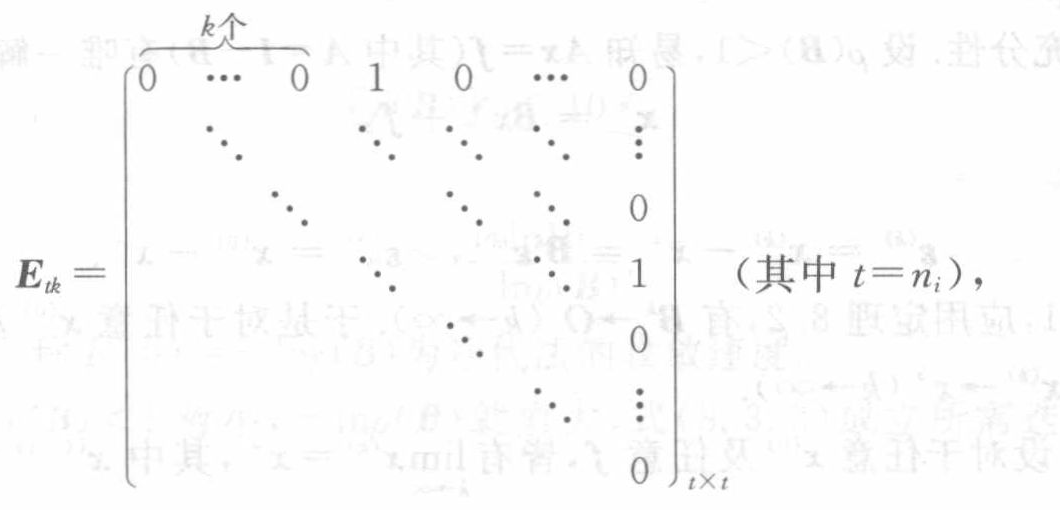
\includegraphics[width=0.85\linewidth,height=\textheight,keepaspectratio,alt={原书无编号矩阵示意：E\_tk}]{verified/assets/ch08/pdf-220-Etk-matrix.png}

原图矩阵符号标签：\(E_{tk}\)，首行前 \(k\) 个元素为零（括注``\(k\) 个''），随后为 \(1,0,\cdots,0\)；第 \(k\) 条上副对角线为 \(1\)，其余为零；矩阵尺寸 \(t\times t\)，其中 \(t=n_i\)。

一般有 \((E_{t1})^k=E_{tk}\)，当 \(k\geqslant t\) 时 \(E_{tk}=O\)。由于

\[
J_i=\begin{bmatrix}
\lambda_i&&&&\\
&\lambda_i&&&\\
&&\ddots&&\\
&&&\ddots&\\
&&&&\lambda_i
\end{bmatrix}
+\begin{bmatrix}
0&1&&&\\
&0&1&&\\
&&\ddots&\ddots&\\
&&&\ddots&1\\
&&&&0
\end{bmatrix}
=\lambda_i I+E_{t1},
\]

\clearpage

原书 PDF 页 221；印刷页码 208。

\href{source-images/pdf-221.jpeg}{原页图像}

于是

\[
\begin{aligned}
J_i^k&=(\lambda_i I+E_{t1})^k
=\sum_{j=0}^k\binom{k}{j}\lambda_i^{k-j}(E_{t1})^j
=\sum_{j=0}^k\binom{k}{j}\lambda_i^{k-j}E_{tj}
=\sum_{j=0}^{t-1}\binom{k}{j}\lambda_i^{k-j}E_{tj}\\[6pt]
&=\begin{bmatrix}
\lambda_i^k&\binom{k}{1}\lambda_i^{k-1}&\cdots&\cdots&\binom{k}{t-1}\lambda_i^{k-(t-1)}\\[5pt]
&\lambda_i^k&\binom{k}{1}\lambda_i^{k-1}&\cdots&\binom{k}{t-2}\lambda_i^{k-(t-2)}\\[5pt]
&&\ddots&\ddots&\vdots\\[5pt]
&&&\ddots&\binom{k}{1}\lambda_i^{k-1}\\[5pt]
&&&&\lambda_i^k
\end{bmatrix}_{t\times t}\quad(i=1,2,\cdots,r),
\end{aligned}
\]

其中

\[
E_{t0}=I,\qquad\binom{k}{j}=\frac{k!}{j!(k-j)!}=\frac{k(k-1)\cdots(k-j+1)}{j!}.
\]

利用极限 \(\lim\limits_{k\to\infty}k^r c^k=0\)（\(0<c<1,r\geqslant0\)），得到

\[
\binom{k}{j}\lambda^{k-j}\to0\quad(k\to\infty)\iff|\lambda|<1,
\]

所以 \(J_i^k\to O\)（\(k\to\infty\)）充要条件是 \(|\lambda_i|<1\)（\(i=1,2,\cdots,r\)），即 \(\rho(B)<1\)。

\textbf{定理 8.3（迭代法基本定理）}　设有方程组

\[
x=Bx+f,
\tag{8.3.1}
\]

对于任意初始向量 \(x^{(0)}\) 及任意 \(f\)，解此方程组的迭代法（即 \(x^{(k+1)}=Bx^{(k)}+f\)）收敛的充要条件是 \(\rho(B)<1\)。

\textbf{证明}　充分性。设 \(\rho(B)<1\)，易知 \(Ax=f\)（其中 \(A=I-B\)）有唯一解，记作

\[
x^*=Bx^*+f.
\tag{8.3.2}
\]

误差向量

\[
\varepsilon^{(k)}=x^{(k)}-x^*=B^k\varepsilon^{(0)},\qquad\varepsilon^{(0)}=x^{(0)}-x^*.
\]

由设 \(\rho(B)<1\)，应用定理 8.2，有 \(B^k\to O\)（\(k\to\infty\)）。于是对于任意 \(x^{(0)}\) 及 \(f\)，有 \(\varepsilon^{(k)}\to0\)（\(k\to\infty\)），即 \(x^{(k)}\to x^*\)（\(k\to\infty\)）。

必要性。设对于任意 \(x^{(0)}\) 及任意 \(f\)，皆有 \(\lim\limits_{k\to\infty}x^{(k)}=x^*\)，其中 \(x^{(k+1)}=Bx^{(k)}+f\)。显然，

（1）极限 \(x^*\) 是方程组（8.3.1）的解，

（2）对于任意 \(x^{(0)}\) 及任意 \(f\)，有

\[
\varepsilon^{(k)}=x^{(k)}-x^*=B^k\varepsilon^{(0)}\to0\quad(k\to\infty).
\]

显然

\[
B^k\to O\quad(k\to\infty).
\]

再由定理 8.2，即得 \(\rho(B)<1\)。

\clearpage

原书 PDF 页 222；印刷页码 209。

\href{source-images/pdf-222.jpeg}{原页图像}

\textbf{例 8.5}　考察用 Jacobi 方法解例 8.1 方程组的收敛性。迭代矩阵 \(B_0\) 的特征方程为

\[
\det(\lambda I-B_0)=\lambda^3+0.034\,090\,909\lambda+0.039\,772\,727=0,
\]

解得

\[
\begin{gathered}
\lambda_1=-0.308\,2,\\
\lambda_2=0.154\,1+\mathrm i0.324\,5,\\
\lambda_3=0.154\,1-\mathrm i0.324\,5,\\
|\lambda_2|=|\lambda_3|=0.359\,2<1,\qquad|\lambda_1|<1,
\end{gathered}
\]

即 \(\rho(B_0)<1\)。所以用 Jacobi 迭代法解方程组（8.3.1）是收敛的。

\textbf{例 8.6}　考察用迭代过程的收敛性：\(x^{(k+1)}=Bx^{(k)}+f\)（\(k=0,1,2,\cdots\)），其中

\[
B=\begin{pmatrix}0&2\\3&0\end{pmatrix},\qquad f=\begin{pmatrix}5\\5\end{pmatrix}.
\]

特征方程为

\[
\det(\lambda I-B)=\lambda^2-6=0,
\]

特征根 \(\lambda_{1,2}=\pm\sqrt6\)，即 \(\rho(B)>1\)。这说明此迭代过程不收敛。

现讨论迭代法的收敛速度。考察误差向量 \(\varepsilon^{(k)}=x^{(k)}-x^*=B^k\varepsilon^{(0)}\)。设 \(B\) 有 \(n\) 个线性无关的特征向量 \(u_1,u_2,\cdots,u_n\)，相应的特征值为 \(\lambda_1,\lambda_2,\cdots,\lambda_n\)。由 \(\varepsilon^{(0)}=\sum\limits_{i=1}^n a_i u_i\)，得

\[
\varepsilon^{(k)}=B^k\varepsilon^{(0)}=\sum_{i=1}^n a_i B^k u_i=\sum_{i=1}^n a_i\lambda_i^k u_i.
\]

可以看出，当 \(\rho(B)<1\) 愈小时，\(\lambda_i^k\to0\)（\(i=1,2,\cdots,n;\ k\to\infty\)）愈快，即 \(\varepsilon^{(k)}\to0\) 愈快，故可用量 \(\rho(B)\) 来刻画迭代法的收敛快慢。现在依据给定精度要求确定迭代次数 \(k\)，即使

\[
[\rho(B)]^k\leqslant10^{-s},
\tag{8.3.3}
\]

取对数得

\[
k\geqslant\frac{s\ln10}{-\ln\rho(B)}.
\]

\textbf{定义 8.3}　称 \(R(B)=-\ln\rho(B)\) 为迭代法的收敛速度。

可以看出，\(\rho(B)<1\) 愈小，\(-\ln\rho(B)\) 就愈大，式（8.3.3）成立所需迭代次数就愈少。

由于一般当 \(n\) 较大时，矩阵特征值计算比较困难，基本定理的条件比较难验证，所以最好建立与矩阵元素直接有关的条件来判别迭代法的收敛性。由于 \(\rho(B)\leqslant\|B\|_v\)（\(v=1,2,\infty\) 或 \(F\)），所以可用 \(\|B\|_v\) 来作为 \(\rho(B)\) 上界的一种估计。

\textbf{定理 8.4（迭代法收敛的充分条件）}　如果方程组（8.3.1）的迭代公式为 \(x^{(k+1)}=Bx^{(k)}+f\)（\(x^{(0)}\) 为任意初始向量），且迭代矩阵的某一种范数 \(\|B\|_v=q<1\)，则：

\(1^\circ\) 迭代法收敛；

\clearpage

原书 PDF 页 223；印刷页码 210。

\href{source-images/pdf-223.jpeg}{原页图像}

\(2^\circ\) \(\|x^*-x^{(k)}\|_v\leqslant\dfrac{q}{1-q}\|x^{(k)}-x^{(k-1)}\|_v\)；

\(3^\circ\) \(\|x^*-x^{(k)}\|_v\leqslant\dfrac{q^k}{1-q}\|x^{(1)}-x^{(0)}\|_v\)。

\textbf{证明}　利用定理 8.3，结论 \(1^\circ\) 是显然的。现证结论 \(2^\circ\)、\(3^\circ\)。据题设显然有

\[
x^*-x^{(k+1)}=B(x^*-x^{(k)}),
\tag{8.3.4}
\]

\[
\|x^{(k+1)}-x^{(k)}\|_v\leqslant q\|x^{(k)}-x^{(k-1)}\|_v\quad(k=1,2,\cdots),
\tag{8.3.5}
\]

\[
\|x^*-x^{(k+1)}\|_v\leqslant q\|x^*-x^{(k)}\|_v.
\tag{8.3.6}
\]

于是

\[
\begin{aligned}
\|x^{(k+1)}-x^{(k)}\|_v
&=\|x^*-x^{(k)}-(x^*-x^{(k+1)})\|_v\\
&\geqslant\|x^*-x^{(k)}\|_v-\|x^*-x^{(k+1)}\|_v\\
&\geqslant(1-q)\|x^*-x^{(k)}\|_v,
\end{aligned}
\]

即

\[
\begin{aligned}
\|x^*-x^{(k)}\|_v
&\leqslant\frac1{1-q}\|x^{(k+1)}-x^{(k)}\|_v\\
&\leqslant\frac{q}{1-q}\|x^{(k)}-x^{(k-1)}\|_v\quad(k=1,2,\cdots).
\end{aligned}
\]

反复利用式（8.3.5）即得到结论 \(3^\circ\)。

\textbf{例 8.7}　仍然考察例 8.1，Jacobi 方法迭代矩阵 \(B_0\) 的 \(\infty\)-范数为

\[
\|B_0\|_\infty=\max\left\{\frac58,\frac5{11},\frac9{12}\right\}=\frac9{12}<1,
\]

所以对例 8.1 应用 Jacobi 迭代方法是收敛的。

\textbf{例 8.8}　设有迭代过程 \(x^{(k+1)}=Bx^{(k)}+f\)（\(k=0,1,2,\cdots\)），其中

\[
B=\begin{pmatrix}0.9&0\\0.3&0.8\end{pmatrix},\qquad f=\begin{pmatrix}1\\2\end{pmatrix},
\]

则

\[
\|B\|_\infty=1.1,\qquad\|B\|_1=1.2,\qquad\|B\|_2=1.021,\qquad\|B\|_F=\sqrt{1.54}.
\]

虽然 \(B\) 的这些范数都大于 1，但 \(B\) 的特征值为 \(\lambda_1=0.9,\lambda_2=0.8\)，由定理 8.3 知，此迭代过程还是收敛的。

由定理 8.4 可知，\(\|B\|=q<1\) 愈小，迭代法收敛愈快。

当 \(B\) 的某一种范数 \(\|B\|<1\) 时，如果相邻两次迭代 \(\|x^{(k)}-x^{(k-1)}\|<\varepsilon_0\)（\(\varepsilon_0\) 为给定的精度要求），则 \(\|x^*-x^{(k)}\|\leqslant\dfrac{q}{1-q}\varepsilon_0\)，所以在用计算机计算时通常利用 \(\|x^{(k)}-x^{(k-1)}\|<\varepsilon_0\) 来作为控制迭代的终止条件。不过要注意，当 \(q\approx1\) 时，\(\dfrac{q}{1-q}\) 较大，尽管 \(\|x^{(k)}-x^{(k-1)}\|\) 已非常小，但误差向量的模 \(\|\varepsilon^{(k)}\|=\|x^*-x^{(k)}\|\) 可能较大，迭代法收敛将是缓慢的。定理 8.4 中结论 \(3^\circ\) 的估计还可以用来事先确定需要迭代多少次才能保证 \(\|\varepsilon^{(k)}\|<\varepsilon_0\)。

\textbf{定理 8.5}　解方程组（8.2.1）的 Gauss-Seidel 迭代法收敛的充要条件是 \(\rho(G)<1\)，

\clearpage

原书 PDF 页 224；印刷页码 211。

\href{source-images/pdf-224.jpeg}{原页图像}

其中 \(G\) 为 Gauss-Seidel 迭代法的迭代矩阵。

\textbf{证明}　由式（8.2.6）再应用定理 8.3 即得定理 8.5。

在实际应用中常遇到一些线性代数方程组，其系数矩阵具有某些性质，如系数矩阵的对角元素占优，系数矩阵为对称正定等。充分利用这些性质往往可使判定迭代法收敛的问题变得简单。

\textbf{定义 8.4（对角占优阵）}　设 \(A=(a_{ij})_{n\times n}\in\mathbb R^{n\times n}\)（或 \(\mathbb C^{n\times n}\)），

\(1^\circ\) 如果矩阵 \(A\) 满足条件

\[
|a_{ii}|>\sum_{\substack{j=1\\j\neq i}}^n|a_{ij}|\quad(i=1,2,\cdots,n),
\tag{8.3.7}
\]

即 \(A\) 的每一行对角元素的绝对值都严格大于同行其他元素绝对值之和，则称 \(A\) 为\textbf{严格对角占优阵}。

\(2^\circ\) 如果 \(|a_{ii}|\geqslant\sum\limits_{\substack{j=1\\j\neq i}}^n|a_{ij}|\)（\(i=1,2,\cdots,n\)）且至少有一个不等式严格成立，称 \(A\) 为\textbf{弱对角占优阵}。

\textbf{例 8.9}　\(A=\begin{bmatrix}-4&1&0&0\\1&-4&1&0\\0&1&-4&1\\0&0&1&-4\end{bmatrix}\) 为严格对角占优阵，\(B=\begin{bmatrix}1&1&0\\1&1&0\\0&1&2\end{bmatrix}\) 为弱对角占优阵。

\textbf{定义 8.5（可约与不可约矩阵）}　设 \(A=(a_{ij})_n\in\mathbb R^{n\times n}\)（或 \(\mathbb C^{n\times n}\)），当 \(n\geqslant2\) 时，如果存在 \(n\) 阶置换阵 \(P\) 使

\[
P^{\mathrm T}AP=\begin{bmatrix}A_{11}&A_{12}\\O&A_{22}\end{bmatrix}
\tag{8.3.8}
\]

成立，其中 \(A_{11}\) 为 \(r\) 阶子矩阵，\(A_{22}\) 为 \(n-r\) 阶子矩阵（\(1\leqslant r\leqslant n\)），则称 \(A\) 是\textbf{可约矩阵}。如果不存在置换阵 \(P\) 使式（8.3.8）成立，则称 \(A\) 是\textbf{不可约矩阵}。

\(A\) 是可约矩阵，意味着 \(Ax=b\) 可经过若干行列重排（若 \(A\) 经过两行交换的同时进行相应的两列的交换，称对 \(A\) 进行一次行列重排），化为两个低阶方程组求解。

事实上，由 \(Ax=b\) 可化为 \(P^{\mathrm T}AP(P^{\mathrm T}x)=P^{\mathrm T}b\)，且记

\[
y=P^{\mathrm T}x=\begin{pmatrix}y_1\\y_2\end{pmatrix},\qquad
P^{\mathrm T}b=\begin{pmatrix}d_1\\d_2\end{pmatrix},
\]

其中 \(y_1,d_1\) 为 \(r\) 维向量。于是，求解 \(Ax=b\) 化为求解

\[
\begin{cases}
A_{11}y_1+A_{12}y_2=d_1,\\
A_{22}y_2=d_2.
\end{cases}
\]

\textbf{例 8.10}　在例 8.9 中矩阵 \(B\) 是可约矩阵，即存在置换阵 \(P=I_{13}\)，使

\begin{quote}
校注（agent 补充）：定义 8.5 的原页范围明确印为 \(1\leqslant r\leqslant n\)，已保留。可约分块需要两个非空低阶方阵，通常应要求 \(1\leqslant r\leqslant n-1\)；若容许 \(r=n\)，第二块阶数为零，定义不能区分可约与不可约。此处疑为原书边界排印错误，并非 OCR 错误。
\end{quote}

\clearpage

原书 PDF 页 225；印刷页码 212。

\href{source-images/pdf-225.jpeg}{原页图像}

\[
P^{\mathrm T}BP=\left[\begin{array}{c|cc}2&1&0\\\hline0&1&1\\0&1&1\end{array}\right].
\]

\textbf{定理 8.6（对角占优定理）}　如果 \(A=(a_{ij})_n\in\mathbb R^{n\times n}\)（或 \(\mathbb C^{n\times n}\)）为严格对角占优阵或为不可约弱对角占优阵，则 \(A\) 是非奇异矩阵。

\textbf{证明}　设 \(A\) 为严格对角占优阵，下面只就这种情况证明此定理。若 \(\det A=0\)，则 \(Ax=0\) 有非零解，记作

\[
x=(x_1,x_2,\cdots,x_n)^{\mathrm T}.
\]

又记 \(|x_k|=\max\limits_{1\leqslant i\leqslant n}|x_i|\neq0\)，由齐次方程组的第 \(k\) 个方程

\[
\sum_{j=1}^n a_{kj}x_j=0,
\]

得

\[
|a_{kk}x_k|=\left|\sum_{\substack{j=1\\j\neq k}}^n a_{kj}x_j\right|
\leqslant\sum_{\substack{j=1\\j\neq k}}^n|a_{kj}|\,|x_j|
\leqslant|x_k|\sum_{\substack{j=1\\j\neq k}}^n|a_{kj}|,
\]

\[
|a_{kk}|\leqslant\sum_{\substack{j=1\\j\neq k}}^n|a_{kj}|,
\tag{8.3.9}
\]

与假设矛盾，故 \(\det A\neq0\)，即 \(A\) 非奇异。

\textbf{定理 8.7}　如果 \(A\in\mathbb R^{n\times n}\) 为严格对角占优阵或为不可约弱对角占优阵，则对于任意的 \(x^{(0)}\)，解方程组（8.2.1）的 Jacobi 迭代法、Gauss-Seidel 迭代法均收敛。

\textbf{证明}　设 \(A\) 为不可约弱对角占优阵，现证明 Gauss-Seidel 迭代法收敛。其他证明留作习题。

由设知 \(a_{ii}\neq0\)（\(i=1,2,\cdots,n\)），方程组（8.2.1）的 Gauss-Seidel 迭代法的迭代矩阵为

\[
G=(D-L)^{-1}U.
\]

又

\[
\begin{aligned}
\det(\lambda I-G)&=\det(\lambda I-(D-L)^{-1}U)\\
&=\det(D-L)^{-1}\cdot\det(\lambda(D-L)-U)=0,
\end{aligned}
\]

即

\[
\det(\lambda(D-L)-U)=0.
\]

记

\[
G=\lambda(D-L)-U=\begin{bmatrix}
\lambda a_{11}&a_{12}&a_{13}&\cdots&a_{1n}\\
\lambda a_{21}&\lambda a_{22}&a_{23}&\cdots&a_{2n}\\
\vdots&\lambda a_{32}&\ddots&\ddots&\vdots\\
\vdots&\vdots&\ddots&\ddots&a_{n-1,n}\\
\lambda a_{n1}&\lambda a_{n2}&\cdots&\lambda a_{n,n-1}&\lambda a_{nn}
\end{bmatrix}=(c_{ij})_{n\times n}.
\]

下面说明当 \(|\lambda|\geqslant1\) 时 \(\det G\neq0\)，如果这个结论是正确的，那么 \(\det G=0\) 的根均满足 \(|\lambda|<1\)。这说明解式（8.2.1）的 Gauss-Seidel 迭代法收敛。

事实上，由 \(A\) 为不可约矩阵，则 \(G\) 亦为不可约矩阵，且又由 \(A\) 为弱对角占优阵得

\begin{quote}
校注（agent 补充）：本页先用 \(G\) 表示 Gauss-Seidel 迭代矩阵，随后在证明中又记 \(G=\lambda(D-L)-U\)。原页第二处字母无上横线或其他修饰，转录保留此符号重用；后面的 \(\det G\) 指随后定义的矩阵。
\end{quote}

\clearpage

原书 PDF 页 226；印刷页码 213。

\href{source-images/pdf-226.jpeg}{原页图像}

到（当 \(|\lambda|\geqslant1\) 时）

\[
|c_{ii}|=|\lambda|\,|a_{ii}|
\geqslant\sum_{j=1}^{i-1}|\lambda a_{ij}|+\sum_{j=i+1}^n|a_{ij}|
=\sum_{j\neq i}|c_{ij}|,
\]

且至少有一不等式严格成立，也就是说当 \(|\lambda|\geqslant1\) 时，\(G\) 为不可约弱对角占优阵，于是由定理 8.6（当 \(|\lambda|\geqslant1\) 时）有 \(\det G\neq0\)，故 \(\rho(G)<1\)。

\subsection{8.4　解线性方程组的超松弛迭代法}\label{ch08-ux89e3ux7ebfux6027ux65b9ux7a0bux7ec4ux7684ux8d85ux677eux5f1bux8fedux4ee3ux6cd5}

逐次超松弛迭代法（successive over relaxation method，简称 SOR 方法）是 Gauss-Seidel 方法的一种加速方法，是解大型稀疏矩阵方程组的有效方法之一，它具有计算公式简单，程序设计容易，占用计算机内存较少等优点，但需要选择好的加速因子（即最佳松弛因子）。

设有方程组

\[
Ax=b,
\tag{8.4.1}
\]

其中 \(A\in\mathbb R^{n\times n}\) 为非奇异矩阵，且设 \(a_{ii}\neq0\)（\(i=1,2,\cdots,n\)），分解 \(A\) 为

\[
A=D-L-U.
\tag{8.4.2}
\]

设已知第 \(k\) 次迭代向量 \(x^{(k)}\)，及第 \(k+1\) 次迭代向量 \(x^{(k+1)}\) 的分量 \(x_j^{(k+1)}\)（\(j=1,2,\cdots,i-1\)），要求计算分量 \(x_i^{(k+1)}\)。

首先用 Gauss-Seidel 迭代法定义辅助量

\[
\tilde{x}_i^{(k+1)}=\frac1{a_{ii}}\left(b_i-\sum_{j=1}^{i-1}a_{ij}x_j^{(k+1)}-\sum_{j=i+1}^{n}a_{ij}x_j^{(k)}\right)\quad(i=1,2,\cdots,n),
\tag{8.4.3}
\]

再把 \(x_i^{(k+1)}\) 取为 \(x_i^{(k)}\) 与 \(\tilde{x}_i^{(k+1)}\) 某个平均值（即加权平均），即

\[
x_i^{(k+1)}=(1-\omega)x_i^{(k)}+\omega\tilde{x}_i^{(k+1)}
=x_i^{(k)}+\omega(\tilde{x}_i^{(k+1)}-x_i^{(k)}).
\tag{8.4.4}
\]

用式（8.4.3）代入式（8.4.4）即得到解方程组 \(Ax=b\) 的逐次超松弛迭代公式

\[
\begin{cases}
x_i^{(k+1)}=x_i^{(k)}+\dfrac{\omega}{a_{ii}}\left(b_i-\displaystyle\sum_{j=1}^{i-1}a_{ij}x_j^{(k+1)}-\displaystyle\sum_{j=i}^n a_{ij}x_j^{(k)}\right),\\[5pt]
x^{(k)}=(x_1^{(k)},x_2^{(k)},\cdots,x_n^{(k)})^{\mathrm T}\quad(k=0,1,\cdots;\ i=1,2,\cdots,n).
\end{cases}
\tag{8.4.5}
\]

其中 \(\omega\) 称为\textbf{松弛因子}，或写为

\[
\begin{cases}
x_i^{(k+1)}=x_i^{(k)}+\Delta x_i\quad(k=0,1,\cdots;\ i=1,2,\cdots,n),\\[5pt]
\Delta x_i=\dfrac{\omega}{a_{ii}}\left(b_i-\displaystyle\sum_{j=1}^{i-1}a_{ij}x_j^{(k+1)}-\displaystyle\sum_{j=i}^n a_{ij}x_j^{(k)}\right).
\end{cases}
\tag{8.4.6}
\]

显然，当 \(\omega=1\) 时，解式（8.4.1）的 SOR 方法就是 Gauss-Seidel 迭代法。

在 SOR 方法中，迭代一次主要的运算量是计算一次矩阵与向量的乘法。由式（8.4.5）可知，在计算机上应用 SOR 方法解方程组时只需一组工作单元，以便存放近似

\clearpage

原书 PDF 页 227；印刷页码 214。

\href{source-images/pdf-227.jpeg}{原页图像}

解。在用计算机计算时，可用 \(|p_0|=\max\limits_i|\Delta x_i|=\max\limits_{1\leqslant i\leqslant n}|x_i^{(k+1)}-x_i^{(k)}|<\varepsilon\) 控制迭代终止。

当 \(\omega<1\) 时，称式（8.4.5）为\textbf{低松弛法}；当 \(\omega>1\) 时，称式（8.4.5）为\textbf{超松弛法}。

\textbf{例 8.11}　用 SOR 方法解方程组

\[
\begin{bmatrix}-4&1&1&1\\1&-4&1&1\\1&1&-4&1\\1&1&1&-4\end{bmatrix}
\begin{bmatrix}x_1\\x_2\\x_3\\x_4\end{bmatrix}
=\begin{bmatrix}1\\1\\1\\1\end{bmatrix},
\]

它的精确解为 \(x^*=(-1,-1,-1,-1)^{\mathrm T}\)。

\textbf{解}　取 \(x^{(0)}=0\)，迭代公式为

\[
\begin{cases}
x_1^{(k+1)}=x_1^{(k)}-\omega(1+4x_1^{(k)}-x_2^{(k)}-x_3^{(k)}-x_4^{(k)})/4,\\
x_2^{(k+1)}=x_2^{(k)}-\omega(1-x_1^{(k+1)}+4x_2^{(k)}-x_3^{(k)}-x_4^{(k)})/4,\\
x_3^{(k+1)}=x_3^{(k)}-\omega(1-x_1^{(k+1)}-x_2^{(k+1)}+4x_3^{(k)}-x_4^{(k)})/4,\\
x_4^{(k+1)}=x_4^{(k)}-\omega(1-x_1^{(k+1)}-x_2^{(k+1)}-x_3^{(k+1)}+4x_4^{(k)})/4.
\end{cases}
\]

取 \(\omega=1.3\)，第 11 次迭代结果为

\[
x^{(11)}=(-0.999\,996\,46,\ -1.000\,003\,10,\ -0.999\,999\,53,\ -0.999\,999\,12)^{\mathrm T},
\]

\[
\|\varepsilon^{(11)}\|_2\leqslant0.46\times10^{-5}.
\]

对 \(\omega\) 取其他值，迭代次数如表 8.1 所示。从此例可以看到，松弛因子选择得好，会使 SOR 方法的收敛大大加速。本例中，\(\omega=1.3\) 是最佳松弛因子。

\Needspace{19\baselineskip}

\textbf{表 8.1}

{\def\LTcaptype{none} % do not increment counter
\begin{longtable}[]{@{}lr@{}}
\toprule\noalign{}
松弛因子 \(\omega\) & 满足误差 \(\|x^{(k)}-x^*\|_2<10^{-5}\) 的迭代次数 \\
\midrule\noalign{}
\endhead
\bottomrule\noalign{}
\endlastfoot
1.0 & 22 \\
1.1 & 17 \\
1.2 & 12 \\
\(\underline{1.3}\) & 11（最少迭代次数） \\
1.4 & 14 \\
1.5 & 17 \\
1.6 & 23 \\
1.7 & 33 \\
1.8 & 53 \\
1.9 & 109 \\
\end{longtable}
}

下面写出 SOR 迭代公式的矩阵形式。迭代公式（8.4.5）亦可写为

\[
a_{ii}x_i^{(k+1)}=(1-\omega)a_{ii}x_i^{(k)}+\omega\left(b_i-\sum_{j=1}^{i-1}a_{ij}x_j^{(k+1)}-\sum_{j=i+1}^n a_{ij}x_j^{(k)}\right)\quad(i=1,2,\cdots,n).
\tag{8.4.7}
\]

用式 \(A=D-L-U\)，则

\[
Dx^{(k+1)}=\omega(b+Lx^{(k+1)}+Ux^{(k)})+(1-\omega)Dx^{(k)},
\]

即

\[
(D-\omega L)x^{(k+1)}=((1-\omega)D+\omega U)x^{(k)}+\omega b.
\]

显然对于任何一个 \(\omega\) 值，\(D-\omega L\) 非奇异（由设 \(a_{ii}\neq0;\ i=1,2,\cdots,n\)），于是

\[
x^{(k+1)}=(D-\omega L)^{-1}[(1-\omega)D+\omega U]x^{(k)}+\omega(D-\omega L)^{-1}b.
\]

这就是说，解式（8.2.1）（设 \(a_{ii}\neq0;\ i=1,2,\cdots,n\)）的 SOR 方法迭代公式为

\[
x^{(k+1)}=L_\omega x^{(k)}+f.
\tag{8.4.8}
\]

\begin{quote}
校注（agent 补充）：原页第 11 次迭代向量及误差界均按原样保留。按所印四个分量计算，\(\|x^{(11)}-x^*\|_2\approx4.8100832\times10^{-6}\)，超过所印上界 \(0.46\times10^{-5}\)。以 \(\omega=13/10\) 从零向量作 11 次有理数迭代，所得向量约为 \((-0.9999966722,-1.0000028727,-0.9999995354,-0.9999991925)^{\mathrm T}\)，误差约为 \(4.4938646\times10^{-6}\)；因此本页所印向量与误差界存在数值不一致，并非 OCR 错误。
\end{quote}

\clearpage

原书 PDF 页 228；印刷页码 215。

\href{source-images/pdf-228.jpeg}{原页图像}

其中

\[
L_\omega=(D-\omega L)^{-1}[(1-\omega)D+\omega U],\qquad f=\omega(D-\omega L)^{-1}b.
\]

矩阵 \(L_\omega\) 称为 SOR 方法的迭代矩阵。这说明对式（8.2.1）应用 SOR 方法相当于对方程组 \(x=L_\omega x+f\) 应用一般迭代法。于是关于一般迭代法的理论可应用到式（8.4.8），得到下述定理。

\textbf{定理 8.8}　设有线性方程组（8.4.1），且 \(a_{ii}\neq0\)（\(i=1,2,\cdots,n\)），则解方程组的 SOR 方法收敛的充要条件是

\[
\rho(L_\omega)<1.
\]

引进超松弛迭代法的想法是希望能选择松弛因子 \(\omega\) 使得迭代过程式（8.4.5）收敛较快，也就是应选择因子 \(\omega\) 使 \(\rho(L_\omega)=\min\limits_\omega\)。

下面研究，对于一般方程组（8.2.1）（\(a_{ii}\neq0;\ i=1,2,\cdots,n\)），松弛因子 \(\omega\) 在什么范围内取值，SOR 方法才可能收敛。现给出 SOR 方法收敛的必要条件。

\textbf{定理 8.9}　设解式（8.2.1）（\(a_{ii}\neq0;\ i=1,2,\cdots,n\)）的 SOR 方法收敛，则

\[
0<\omega<2.
\]

\textbf{证明}　由设 SOR 方法收敛，根据定理 8.8，\(\rho(L_\omega)<1\)。

设 \(L_\omega\) 的特征值为 \(\lambda_1,\lambda_2,\cdots,\lambda_n\)，则

\[
|\det L_\omega|=|\lambda_1\lambda_2\cdots\lambda_n|\leqslant(\rho(L_\omega))^n,\qquad
|\det L_\omega|^{1/n}\leqslant\rho(L_\omega)<1.
\]

而

\[
\det L_\omega=\det((D-\omega L)^{-1})\cdot\det((1-\omega)D+\omega U)=(1-\omega)^n,
\]

所以

\[
|1-\omega|<1.
\]

该定理说明对于解一般方程组（8.2.1）（\(a_{ii}\neq0;\ i=1,2,\cdots,n\)），SOR 方法只有取松弛因子 \(\omega\) 在 \((0,2)\) 范围内才能收敛。而当 \(A\) 是对称正定矩阵时，若 \(\omega\) 满足 \(0<\omega<2\)，则 SOR 方法一定收敛。

\textbf{定理 8.10}　如果 \(A\) 为对称正定矩阵，且 \(0<\omega<2\)，则解式（8.4.1）的 SOR 方法收敛。

\textbf{证明}　在上述假定下，若能证明 \(|\lambda|<1\)，那么定理得证（其中 \(\lambda\) 为 \(L_\omega\) 的任一特征值）。

事实上，设 \(y\) 为对应 \(\lambda\) 的 \(L_\omega\) 的特征向量，即

\[
L_\omega y=\lambda y,\qquad y=(y_1,y_2,\cdots,y_n)^{\mathrm T}\neq0,
\]

\[
(D-\omega L)^{-1}[(1-\omega)D+\omega U]y=\lambda y,
\]

亦即

\[
[(1-\omega)D+\omega U]y=\lambda(D-\omega L)y.
\]

为了找出 \(\lambda\) 的表达式，考虑数量积

\[
(((1-\omega)D+\omega U)y,y)=\lambda((D-\omega L)y,y),
\]

则

\[
\lambda=\frac{(Dy,y)-\omega(Dy,y)+\omega(Uy,y)}{(Dy,y)-\omega(Ly,y)},
\]

\clearpage

原书 PDF 页 229；印刷页码 216。

\href{source-images/pdf-229.jpeg}{原页图像}

显然

\[
(Dy,y)=\sum_{i=1}^n a_{ii}|y_i|^2\equiv\sigma>0,
\tag{8.4.9}
\]

记 \(-(Ly,y)=\alpha+\mathrm i\beta\)，由于 \(A=A^{\mathrm T}\)，所以 \(U=L^{\mathrm T}\)。

\[
-(Uy,y)=-(y,Ly)=-\overline{(Ly,y)}=\alpha-\mathrm i\beta,
\]

\[
0<(Ay,y)=((D-L-U)y,y)=\sigma+2\alpha,
\tag{8.4.10}
\]

所以

\[
\lambda=\frac{(\sigma-\omega\sigma-\alpha\omega)+\mathrm i\omega\beta}{(\sigma+\alpha\omega)+\mathrm i\omega\beta},
\]

从而

\[
|\lambda|^2=\frac{(\sigma-\omega\sigma-\alpha\omega)^2+\omega^2\beta^2}{(\sigma+\alpha\omega)^2+\omega^2\beta^2}.
\]

当 \(0<\omega<2\) 时，利用式（8.4.9）、式（8.4.10），有

\[
(\sigma-\omega\sigma-\alpha\omega)^2-(\sigma+\alpha\omega)^2
=\omega\sigma(\sigma+2\sigma)(\omega-2)<0,
\]

即 \(L_\omega\) 的任一特征值满足 \(|\lambda|<1\)，故 SOR 方法收敛。注意，当 \(0<\omega<2\) 时，可以证明

\[
(\sigma+2\omega)^2+\omega^2\beta^2\neq0.
\]

最佳松弛因子理论是由 Young（1950 年）针对一类椭圆型微分方程数值解得到的代数方程组 \(Ax=b\)（具有所谓性质 A 和相容次序）所建立的理论。他给出了最佳松弛因子公式

\[
\omega_{\mathrm{opt}}=\frac2{1+\sqrt{1-\rho^2(B_0)}},
\]

其中 \(\rho(B_0)\) 是 Jacobi 方法迭代矩阵 \(B_0\) 的谱半径。

一般来说，在实际应用中计算 \(\rho(B_0)\) 较困难，对某些微分方程数值解问题可考虑用第 9 章求近似值的方法，亦可由计算实践摸索出（近似）最佳松弛因子。

\textbf{算法}　本算法用 SOR 方法解式（8.2.1），其中 \(A\) 为对称正定矩阵。数组 \(x\) 为一组工作单元，开始存放初始向量，然后存放近似值解 \(x^{(k)}\)，最后存放结果。用

\[
|p_0|=\max_{1\leqslant i\leqslant n}|\Delta x_i|=\max_{1\leqslant i\leqslant n}|x_i^{(k+1)}-x_i^{(k)}|<\varepsilon\quad\text{（精度要求）}
\]

控制迭代终止。\(k\) 表示迭代次数，可以不用。

\textbf{步 1}　\(k\leftarrow0\)。

\textbf{步 2}　\(x_i\leftarrow0\)（\(i=1,2,\cdots,n\)）。

\textbf{步 3}　\(k\leftarrow k+1\)。

\textbf{步 4}　\(p_0\leftarrow0\)。

\textbf{步 5}　对于 \(i=1,2,\cdots,n\)，有

（1）\(p\leftarrow\Delta x_i=\omega\left(b_i-\displaystyle\sum_{j=1}^{i-1}a_{ij}x_j-\displaystyle\sum_{j=i+1}^n a_{ij}x_j\right)/a_{ii}\)；

（2）如果 \(|p|>|p_0|\)，则 \(p_0\leftarrow p\)；

（3）\(x_i\leftarrow x_i+p\)。

\textbf{步 6}　输出 \(p_0\)。

\begin{quote}
校注（agent 补充）：本页存在以下三处疑似原书排印错误，均已放大核对并保留原式，并非 OCR 错误。第一，平方差的因子原印 \(\sigma+2\sigma\)，代数展开应得 \(\sigma+2\alpha\)，与式（8.4.10）一致。第二，分母非零说明原印 \((\sigma+2\omega)^2+\omega^2\beta^2\neq0\)，由上文 \(|\lambda|^2\) 表达式，相应分母应为 \((\sigma+\alpha\omega)^2+\omega^2\beta^2\)。第三，算法步 5（1）的第二个求和下限原印 \(j=i+1\)；由于随后执行 \(x_i\leftarrow x_i+p\)，\(p=\Delta x_i\) 应是校正量，对照式（8.4.6），该下限应为 \(j=i\)（或另减去 \(a_{ii}x_i\)），否则漏掉对角项。
\end{quote}

\clearpage

原书 PDF 页 230；印刷页码 217。

\href{source-images/pdf-230.jpeg}{原页图像}

\textbf{步 7}　如果 \(|p_0|>\varepsilon\)，则转步 3。

\textbf{步 8}　输出结果 \(x,k\)。

\subsection{小结}\label{ch08-ux5c0fux7ed3}

本章介绍了解线性方程组 \(Ax=b\) 迭代法的一些基本理论及 Jacobi 迭代法、Gauss-Seidel 迭代法、SOR 迭代法，这三种方法都是一阶定常迭代法。在应用中 SOR 方法较为重要，它是解大型稀疏矩阵方程组的有效方法之一。

迭代法是一种逐次逼近方法，在使用迭代法解方程组时，其系数矩阵在计算过程中始终不变。

迭代法具有循环的计算公式，方法简单，适宜解大型稀疏矩阵方程组，在用计算机计算时只需存储 \(A\) 的非零元素（或可按一定公式形成系数，这样 \(A\) 就不需要存储）。

在使用迭代法时，要注意收敛性及收敛速度问题，使用 SOR 方法要选择较佳松弛因子。

迭代法的进一步学习，读者可参看文献{[}11{]}、{[}15{]}、{[}16{]}。

\subsection{习题}\label{ch08-ux4e60ux9898}

\textbf{1.} 设方程组

\[
\begin{cases}
5x_1+2x_2+x_3=-12,\\
-x_1+4x_2+2x_3=20,\\
2x_1-3x_2+10x_3=3.
\end{cases}
\]

（1）考察用 Jacobi 迭代法、Gauss-Seidel 迭代法解此方程组的收敛性；

（2）用 Jacobi 迭代法、Gauss-Seidel 迭代法解此方程组，要求当 \(\|x^{(k+1)}-x^{(k)}\|_\infty<10^{-4}\) 时迭代终止。

\textbf{2.} 设 \(A=\begin{pmatrix}0&0\\2&0\end{pmatrix}\)，证明即使 \(\|A\|_1=\|A\|_\infty>1\)，级数 \(I+A+A^2+\cdots+A^k+\cdots\) 也收敛。

\textbf{3.} 证明对于任意选择的 \(A\)，序列 \(I,\allowbreak A,\allowbreak \dfrac12A^2,\allowbreak \dfrac1{3!}A^3,\allowbreak \dfrac1{4!}A^4,\allowbreak \cdots\) 收敛于零。

\textbf{4.} 设方程组

\[
\begin{cases}
a_{11}x_1+a_{12}x_2=b_1,\\
a_{21}x_1+a_{22}x_2=b_2
\end{cases}
\quad(a_{11}\cdot a_{22}\neq0).
\]

迭代公式为

\[
\begin{cases}
x_1^{(k)}=\dfrac1{a_{11}}(b_1-a_{12}x_2^{(k-1)}),\\[5pt]
x_2^{(k)}=\dfrac1{a_{22}}(b_2-a_{21}x_1^{(k-1)})
\end{cases}
\quad(k=1,2,\cdots).
\]

求证：由上述迭代公式产生的向量序列 \(\{x^{(k)}\}\) 收敛的充要条件是 \(r=\left|\dfrac{a_{12}a_{21}}{a_{11}a_{22}}\right|<1\)。

\textbf{5.} 设方程组

\clearpage

原书 PDF 页 231；印刷页码 218。

\href{source-images/pdf-231.jpeg}{原页图像}

（1）

\[
\begin{cases}
x_1+0.4x_2+0.4x_3=1,\\
0.4x_1+x_2+0.8x_2=2,\\
0.4x_1+0.8x_2+x_3=3;
\end{cases}
\]

（2）

\[
\begin{cases}
x_1+2x_2-2x_3=1,\\
x_1+x_2+x_3=1,\\
2x_1+2x_2+x_3=1.
\end{cases}
\]

试考察解此方程组的 Jacobi 迭代法及 Gauss-Seidel 迭代法的收敛性。

\textbf{6.} 求证 \(\lim\limits_{k\to\infty}A_k=A\) 的充要条件是，对于任何向量 \(x\) 都有 \(\lim\limits_{k\to\infty}A_kx=Ax\)。

\textbf{7.} 设 \(Ax=b\)，其中 \(A\) 为对称正定矩阵，问解此方程组的 Jacobi 迭代法是否一定收敛。试考察习题 5 中方程组（1）。

\textbf{8.} 设方程组

\[
\begin{cases}
x_1-\dfrac14x_3-\dfrac14x_4=\dfrac12,\\[5pt]
x_2-\dfrac14x_3-\dfrac14x_4=\dfrac12,\\[5pt]
-\dfrac14x_1-\dfrac14x_2+x_3=\dfrac12,\\[5pt]
-\dfrac14x_1-\dfrac14x_2+x_4=\dfrac12.
\end{cases}
\]

（1）求解此方程组的 Jacobi 迭代法的迭代矩阵 \(B_0\) 的谱半径；

（2）求解此方程组的 Gauss-Seidel 迭代法的迭代矩阵 \(B_0\) 的谱半径；

（3）考察解此方程组的 Jacobi 迭代法及 Gauss-Seidel 迭代法的收敛性。

\textbf{9.} 用 SOR 方法解方程组（分别取松弛因子 \(\omega=1.03,\omega=1,\omega=1.1\)）

\[
\begin{cases}
4x_1-x_2=1,\\
-x_1+4x_2-x_3=4,\\
-x_2+4x_3=-3.
\end{cases}
\]

精确解 \(x^*=\left(\dfrac12,1,-\dfrac12\right)^{\mathrm T}\)，要求当 \(\|x^*-x^{(k)}\|_\infty<5\times10^{-6}\) 时迭代终止，并且对每一个 \(\omega\) 值确定迭代次数。

\textbf{10.} 用 SOR 方法解方程组（取 \(\omega=0.9\)）

\[
\begin{cases}
5x_1+2x_2+x_3=-12,\\
-x_1+4x_2+2x_3=20,\\
2x_1-3x_2+10x_3=3,
\end{cases}
\]

要求当 \(\|x^{(k+1)}-x^{(k)}\|_\infty<10^{-4}\) 时迭代终止。

\textbf{11.} 设有方程组 \(Ax=b\)，其中 \(A\) 为对称正定矩阵，迭代公式 \(x^{(k+1)}=x^{(k)}+\omega(b-Ax^{(k)})\)（\(k=0,1,2,\cdots\)），试证明当 \(0<\omega<\dfrac2\beta\) 时上述迭代法收敛（其中 \(0<\alpha\leqslant\lambda(A)\leqslant\beta\)）。

\textbf{12.} 用 Gauss-Seidel 方法解 \(Ax=b\)，用 \(x_i^{(k+1)}\) 记 \(x^{(k+1)}\) 的第 \(i\) 个分量，且

\[
r_i^{(k+1)}=b_i-\sum_{j=1}^{i-1}a_{ij}x_j^{(k+1)}-\sum_{j=i}^n a_{ij}x_i^{(k)}.
\]

（1）证明 \(x_i^{(k+1)}=x_i^{(k)}+\dfrac{r_i^{(k+1)}}{a_{ii}}\)；

（2）如果 \(\varepsilon^{(k)}=x^{(k)}-\lambda^*\)，其中 \(x^*\) 是方程组的精确解，求证：\(\varepsilon_i^{(k+1)}=\varepsilon_i^{(k)}-\dfrac{r_i^{(k+1)}}{a_{ii}}\)，其中

\begin{quote}
校注（agent 补充）：习题 5（1）第二行原页确印 \(0.4x_1+x_2+0.8x_2=2\)，已保留。第 7 题将该方程组作为对称正定系数矩阵的考察对象；若将最后一项改为 \(0.8x_3\) 才与该对称结构一致，故此处疑为原书下标错误。

校注（agent 补充）：习题 8（2）的 Gauss-Seidel 迭代矩阵原页也记为 \(B_0\)，与（1）的 Jacobi 迭代矩阵符号相同，转录保留。

校注（agent 补充）：习题 12 有三处原书疑误，均经放大目视后原样保留。残差定义第二个求和内确印 \(x_i^{(k)}\)，对照 Gauss-Seidel 校正量应为 \(x_j^{(k)}\)；（2）的误差定义确印 \(x^{(k)}-\lambda^*\)，而紧随其后说明的是精确解 \(x^*\)；若误差定义按 \(\varepsilon^{(k)}=x^{(k)}-x^*\) 理解，则由（1）可知递推中的校正项应为加号，原题所印减号与此前定义不一致。这里仅定位符号矛盾，不代做习题证明。
\end{quote}

\clearpage

原书 PDF 页 232；印刷页码 219。

\href{source-images/pdf-232.jpeg}{原页图像}

\[
r_i^{(k+1)}=\sum_{j=1}^{i-1}a_{ij}\varepsilon_j^{(k+1)}+\sum_{j=i}^n a_{ij}\varepsilon_j^{(k)};
\]

（3）设 \(A\) 是对称的，二次型 \(Q(\varepsilon^{(k)})=(A\varepsilon^{(k)},\varepsilon^{(k)})\)，证明

\[
Q(\varepsilon^{(k+1)})-Q(\varepsilon^{(k)})=-\sum_{j=1}^n\frac{(r_j^{(k+1)})^2}{a_{jj}}.
\]

（4）由此推出，如果 \(A\) 是具有正对角元素的非奇异矩阵，且 Gauss-Seidel 方法对于任意初始向量 \(x^{(0)}\) 是收敛的，则 \(A\) 是正定矩阵。

\textbf{13.} 设 \(A\) 与 \(B\) 为 \(n\) 阶矩阵，\(A\) 为非奇异矩阵，考虑解方程组 \(Az_1+Bz_2=b_1\)，\(Bz_1+Az_2=b_2\)，其中 \(z_1,z_2,b_1,b_2\in\mathbb R^n\)。

（1）找出下述迭代方法收敛的充要条件

\[
Az_1^{(m+1)}=b_1-Bz_2^{(m)},\qquad Az_2^{(m+1)}=b_2-Bz_1^{(m)}\quad(m\geqslant0);
\]

（2）找出下述迭代方法收敛的充要条件

\[
Az_1^{(m+1)}=b_1-Bz_2^{(m)},\qquad Az_2^{(m+1)}=b_2-Bz_1^{(m+1)}\quad(m\geqslant0).
\]

比较两个方法的收敛速度。

\textbf{14.} 证明矩阵 \(A=\begin{bmatrix}1&a&a\\a&1&a\\a&a&1\end{bmatrix}\) 对于 \(-\dfrac12<a<1\) 是正定的，而 Jacobi 迭代只对 \(-\dfrac12<a<\dfrac12\) 是收敛的。

\textbf{15.} 设 \(A=\begin{bmatrix}5&1&2&3\\0&2&0&4\\3&-1&2&-1\\0&3&0&7\end{bmatrix}\)，试说明 \(A\) 为可约矩阵。

\textbf{16.} 给定迭代过程 \(x^{(k+1)}=Cx^{(k)}+g\)，其中 \(C\in\mathbb R^{n\times n}\)（\(k=0,1,2,\cdots\)），试证明：如果 \(C\) 的特征值 \(\lambda_i(C)=0\)（\(i=1,2,\cdots,n\)），则此迭代过程最多迭代 \(n\) 次收敛于方程组的解。

\textbf{17.} 画出 SOR 方法的框图。

\textbf{18.} 设 \(A\) 为不可约弱对角占优阵且 \(0<\omega\leqslant1\)，求证，解 \(Ax=b\) 的 SOR 方法收敛。

\textbf{19.} 设 \(Ax=b\)，其中 \(A\) 为非奇异矩阵。

（1）求证 \(A^{\mathrm T}A\) 为对称正定矩阵；

（2）求证 \(\operatorname{cond}(A^{\mathrm T}A)_2=(\operatorname{cond}(A)_2)^2\)。

\textbf{20.} 设 \(A\) 为严格对角占优阵，证明式（2.8.23）。

\begin{quote}
校注（agent 补充）：页首为习题 12（2）的续式。该残差表达式中的正号与上页所印误差定义 \(\varepsilon^{(k)}=x^{(k)}-\lambda^*\) 不一致；若误差定义取 \(x^*-x^{(k)}\)，则可与此续式及上页的减号递推一致。两页原文均保留，详见上页习题 12 校注。
\end{quote}

